%% Computer Standards & Interfaces (Elsevier) -- els-cas-templates, double column.
%% Compile with pdfLaTeX + BibTeX (Overleaf: default settings).
%% Items still to complete are marked TODO (search for it).
\documentclass[a4paper,fleqn]{cas-dc}

\usepackage[numbers,sort&compress]{natbib}
\usepackage{booktabs,tabularx,array}
\usepackage[inline]{enumitem}
\usepackage{listings}
\usepackage{tikz}
\usetikzlibrary{positioning,arrows.meta,calc}
\usepackage{newunicodechar}
\usepackage{url}

\setlength{\emergencystretch}{3em}
\def\UrlBreaks{\do\.\do\_\do\-\do\/\do\,\do\(\do\)\do\'\do\:}
\Urlmuskip=0mu plus 0.5mu
\newcolumntype{L}{>{\raggedright\arraybackslash}X}
\newunicodechar{−}{\ensuremath{-}}
\newunicodechar{λ}{\ensuremath{\lambda}}

\lstdefinestyle{json}{basicstyle=\ttfamily\scriptsize, columns=fullflexible,
  breaklines=true, frame=single, rulecolor=\color{black!30}, xleftmargin=2pt,
  xrightmargin=2pt, aboveskip=3pt, belowskip=0pt, showstringspaces=false}

% pandoc output uses these two macros
\providecommand{\tightlist}{\setlength{\itemsep}{0pt}\setlength{\parskip}{0pt}}
\def\pandocbounded#1{#1}

\begin{document}
\let\WriteBookmarks\relax
\def\floatpagepagefraction{1}
\def\textpagefraction{.001}

\shorttitle{Verifiable compliance evidence for high-risk AI}
\shortauthors{D.R. Carneiro et al.}

\title [mode = title]{Verifiable, minimally disclosed compliance evidence for high-risk AI: signed evidence chains, OSCAL and Hyperledger Fabric under the EU AI Act}

% TODO: ORCID of each author, as [orcid=0000-0000-0000-0000] after the name.
\author[1,2]{Davide Rua Carneiro}
\cormark[1]
\ead{dcarneiro@estg.ipp.pt}

% TODO: confirm Rui Sousa's affiliation.
\author[3]{Rui Pedro Teixeira de Sousa}

\author[1]{Guilherme Palumbo}

\author[2]{Diogo Torres}

\affiliation[1]{organization={CIICESI, School of Technology and Management, Technical University of Porto},
  postcode={4610-156}, city={Felgueiras}, country={Portugal}}
\affiliation[2]{organization={INESC TEC}, addressline={Rua Dr. Roberto Frias},
  postcode={4200-465}, city={Porto}, country={Portugal}}
\affiliation[3]{organization={School of Technology and Management, Technical University of Porto},
  postcode={4610-156}, city={Felgueiras}, country={Portugal}}

\cortext[1]{Corresponding author}

\begin{abstract}
The EU AI Act requires providers of high-risk AI systems to demonstrate compliance through records, yet the records that machine-learning pipelines keep can only be vouched for by whoever produced them. We present and evaluate a compliance-as-code architecture that turns AI Act obligations into evidence records a third party can verify. A derivation method maps seven provisions to pipeline requirements, evidence and mechanisms, and states for each what the evidence does not establish. A Compliance Policy Engine issues Ed25519-signed, hash-chained records in RFC 8785 canonical form, exports them as OSCAL 1.1.2 assessment results with selective disclosure for Art.~78, and anchors them on Hyperledger Fabric per record or in Merkle batches. We evaluate the artefact on canonical scenarios, a credit-scoring pipeline, an industrial data stream, a four-arm ablation, a Fabric network and fourteen audit questions. A verifiable log adds 0.068\,ms per event to a database row, of which the signature takes 0.017\,ms. On the ledger, every transaction waits for the orderer's batch timeout, and batching raises durable throughput from 0.49 to 245 records per second at the default timeout. Signatures detect any alteration of a record, an external anchor adds truncation and insider rewriting up to the last anchor, and no configuration detects events withheld or forged at the source. The evidence establishes the integrity and provenance of recorded decisions, not their truth or legal sufficiency. OSCAL catalogues for the AI Act and canonical JSON with cross-implementation conformance tests would make such evidence portable.
\end{abstract}

\begin{highlights}
\item AI Act obligations mapped to evidence records with explicit evidentiary limits
\item Signing costs little; ledger cost lies in distributed ordering
\item Batched anchoring trades audit granularity for durable-evidence throughput
\item OSCAL selective disclosure preserves integrity anchors for Art. 78 audits
\item Evaluated on real credit-scoring and industrial data streams
\end{highlights}

\begin{keywords}
EU AI Act \sep compliance-as-code \sep tamper-evident logging \sep OSCAL \sep Hyperledger Fabric \sep MLOps \sep selective disclosure
\end{keywords}

\maketitle

\section{Introduction}
\label{sec:introduction}

The AI Act~\cite{ai_act} moves the providers of high-risk AI systems from declared to demonstrable compliance. Systems listed in its Annex III, such as creditworthiness assessment, recruitment and access to essential services, must meet requirements that can only be shown through records: technical documentation kept up to date (Art.~11 and Annex~IV), automatic logging of events over the system's lifetime (Art.~12), human oversight (Art.~14), post-market monitoring (Art.~72) and the reporting of serious incidents (Art.~73). Whoever supervises such a system will read those records and act on them.

The records that machine-learning pipelines keep were not made for that reader. MLOps tools log for operational observability: their records are mutable, held by the organisation that produces them, and not linked to any obligation. A human approval is a flag in a database, not a statement with a verifiable author. An external auditor who receives such records must trust the party under audit to have kept them intact, which is the old problem of the integrity of the witness.

The timing makes the problem practical. Regulation (EU) 2026/1744~\cite{omnibus_2026} set the application of the Annex III requirements to 2 December 2027 and of those under Art.~6(1) to 2 August 2028, and left the duties on logging, oversight, accuracy and incident reporting as they were. Implementing Regulation (EU) 2025/2531~\cite{qel_2025} fixed the reference standards for qualified electronic ledgers under eIDAS. The European Data Protection Board adopted the final version of its guidelines on blockchain in July 2026~\cite{edpb_2026}. And the new product liability directive~\cite{pld_2024}, which covers software, applies to products placed on the market after 9 December 2026, with a duty to disclose evidence in litigation.

The technical pieces exist, but apart. Tamper-evident logging is mature, from secure audit logs~\cite{schneier1999} and history trees~\cite{crosby2009} to Certificate Transparency~\cite{rfc9162}, yet it is not tied to legal obligations. Work aimed at the AI Act maps obligations to controls and documentation~\cite{lucaj2025,ugarte2026,buscemi2026,palumbo2025,ramos2024}, yet none of it signs or anchors the evidence when the pipeline produces it. Among the works we reviewed, none states what its evidence does not establish, and none measures where the cost of verifiable evidence lies.

This article joins the two lines. Following design science research with an artificial ex post evaluation, it presents a compliance-as-code architecture that turns AI Act obligations into evidence records a third party can verify, produced as a by-product of the pipeline. It answers three research questions:
\begin{description}[leftmargin=0pt, itemsep=2pt]
\item[RQ1.] How can AI Act obligations for high-risk systems be translated into evidence records that third parties can verify, and what does each record fail to establish?
\item[RQ2.] Which integrity, minimisation and selective-disclosure guarantees can such records offer, and which threats remain outside them?
\item[RQ3.] What does verifiable evidence cost, and where does the cost lie: in cryptography, in persistence or in distributed coordination?
\end{description}

The article makes five contributions.
\begin{enumerate}[label=C\arabic*., leftmargin=*, itemsep=2pt]
\item A derivation method from obligation to pipeline requirement, evidence and mechanism, applied to seven provisions in a matrix with an explicit column on what each record does not establish, and an evidence model that commits to the artefact, keeps the inputs of each decision and correlates the events of a run (Section~\ref{sec:derivation}).
\item A Compliance Policy Engine with fail-closed validation, a closed rule vocabulary, policies archived by hash and decisions that can be re-executed from the record, writing Ed25519-signed, hash-chained records (Section~\ref{sec:architecture}).
\item An OSCAL 1.1.2 profile of assessment results that separates technical objectives from legal provisions, with a redacted mode for Art.~78 that keeps the integrity anchors (Section~\ref{sec:architecture}).
\item An evaluation that locates the cost: a four-arm ablation, per-record and batched anchoring on Hyperledger Fabric, a credit-scoring pipeline on real data, an industrial data stream, a tamper experiment and fourteen audit questions (Section~\ref{sec:evaluation}).
\item Interoperability lessons from eight defects found between the Python issuer and the Go chaincode, and a shared boundary matrix that works as a conformance test (Section~\ref{sec:eval-interop}).
\end{enumerate}

The artefact extends the prototype of a master's dissertation~\cite{sousa2026}. The second version of the evidence model, its canonical form, signed approvals, batched anchoring and every experiment reported here are new to this article.

The scope is deliberately narrow. The evidence establishes the integrity and provenance of what was recorded; it does not establish that the system complies with the AI Act, that the recorded metrics were true, that no event was withheld, or that a court would give the records any particular weight. Section~\ref{sec:background} reviews related work, Section~\ref{sec:approach} sets out the research approach, Section~\ref{sec:derivation} derives the evidence from the obligations, Section~\ref{sec:architecture} describes the architecture and Section~\ref{sec:evaluation} evaluates it. Section~\ref{sec:discussion} discusses what the results mean, Section~\ref{sec:threats} the threats to their validity, and Section~\ref{sec:conclusion} concludes.

\section{Background and related work}
\label{sec:background}

Tamper-evident logging and the normative mapping of AI regulation have matured separately. Logging research offers integrity that a third party can check, without reference to legal obligations; AI Act compliance research offers the mapping, without integrity that anyone but the producer can vouch for. This section reviews both lines and shows where they fail to meet.

\subsection{The AI Act's evidence-bearing obligations}

Regulation (EU) 2024/1689 (the AI Act)~\cite{ai_act} sets requirements for high-risk AI systems that can only be demonstrated through records. For the systems listed in Annex III, which include creditworthiness assessment, employment and access to essential services, the requirements of Chapter III apply from 2 December 2027. For high-risk systems under Art. 6(1) and Annex I they apply from 2 August 2028. Both dates were set by Regulation (EU) 2026/1744~\cite{omnibus_2026}, which amended Art. 113 AI Act.

That amendment changed little of what this article relies on. It extended simplified technical documentation to small mid-cap enterprises (Art. 11(1)), replaced the post-market monitoring template of Art. 72(3) with Commission guidance, and amended Art. 10(1), (5) and (6). It left untouched the provisions on bias examination and data quality used here, Art. 10(2)(f)--(g) and 10(3), and Arts. 12, 14, 15, 19, 73 and 78. Table~\ref{tab:obligations} lists the obligations that presuppose a record, what that record must show, and who reads it.

\begin{table*}[t]
\caption{AI Act obligations that presuppose a record, as amended by Regulation (EU) 2026/1744.}
\label{tab:obligations}
\footnotesize
\begin{tabularx}{\textwidth}{@{}>{\raggedright\arraybackslash}p{0.15\textwidth}LL@{}}
\toprule
Provision & Record that must exist & Who reads it \\
\midrule
Art. 10(2)(f)--(g), 10(3) & Examination of possible biases and the measures taken; relevance, representativeness and completeness of training, validation and test data & Provider; market surveillance authority on request (Art. 74(12)); notified body (Annex VII, 4.3) \\
Art. 11, Annex IV & Technical documentation kept up to date, including the data, metrics and validation procedures (Annex IV, 2(d), 2(g)) and the post-market monitoring plan (Annex IV, 9) & Market surveillance authority; notified body \\
Art. 12 & Automatic recording of events over the system's lifetime, sufficient to identify risk situations, support post-market monitoring and monitor operation & Provider; deployer (Art. 26(5)); authority on reasoned request (Art. 21(2)) \\
Art. 14 & Measures that let natural persons oversee the system, including deciding not to use, overriding or stopping it (Art. 14(4)) & Deployer; market surveillance authority \\
Art. 15 & Declared levels of accuracy and the metrics behind them (Art. 15(3)); robustness and cybersecurity measures & Deployer, through the instructions for use; market surveillance authority \\
Art. 19 & Retention by the provider of the automatically generated logs for at least six months & Provider; market surveillance authority \\
Art. 72 & Post-market monitoring that collects and analyses performance data, based on a plan & Provider; market surveillance authority \\
Art. 73 & Report of each serious incident within the deadlines of Art. 73(2)--(4) & Market surveillance authority \\
Art. 78 & Confidentiality of the information obtained, protecting trade secrets and source code & Binds the readers above \\
\bottomrule
\end{tabularx}
\end{table*}


The typical reader of this evidence is a market surveillance authority, not a notified body. For most Annex III systems the provider follows the internal control procedure of Annex VI (Art. 43(2)); notified bodies intervene only in the cases of Art. 43(1) and under the sectoral procedures for Annex I products. For credit institutions the authority is the financial supervisor (Art. 74(6)). Either way, the reader did not produce the evidence and must decide how far to trust whoever did. That is the problem this article addresses.

\subsection{Tamper-evident logging and ledger anchoring}

Making the alteration of a record detectable is an old problem with standard answers. Haber and Stornetta~\cite{haber1991} linked each timestamp to its predecessor through a hash, so that a back-dated insertion breaks the chain. Schneier and Kelsey~\cite{schneier1999} designed audit logs for an untrusted machine whose entries made before a compromise cannot be read or altered undetected. Crosby and Wallach~\cite{crosby2009} replaced the linear chain with a history tree built on Merkle trees~\cite{merkle1987}, giving logarithmic proofs that an entry is in the log and that one version of the log extends another.

Transparency logs put these structures into production. Certificate Transparency (RFC 9162)~\cite{rfc9162} publishes certificates in append-only Merkle logs whose signed tree heads let monitors detect a log that rewrites or forks its history. Sigstore applies the same design to software signing through its Rekor log~\cite{newman2022}. Trusted timestamping (RFC 3161)~\cite{rfc3161} adds a third party's attestation that data existed at a given time. None of these needs a blockchain: integrity follows from hashing, signatures and the publication of a commitment the log operator cannot retract.

Permissioned ledgers add governance over who may write, and in what order. Hyperledger Fabric~\cite{androulaki2018} separates execution, ordering and validation. Chaincode runs on endorsing peers, an ordering service sequences transactions into blocks, and each peer checks them against an endorsement policy before committing. Identities come from Membership Service Providers (MSPs), so every transaction names the organisation that submitted it. Fabric's ordering service uses Raft~\cite{ongaro2014}, which tolerates crash faults but not Byzantine ones; integrity against a faulty orderer rests on the endorsement policy and on each organisation keeping its own copy of the ledger.

Several works build audit trails on such ledgers. Regueiro et al.~\cite{regueiro2021} implement a blockchain audit trail that improves on the security and usability of conventional audit-log solutions. Lu et al.~\cite{lu2020} and Shi et al.~\cite{shi2022} build integrity-verification trails over Fabric, and Sychowiec and Zieliński~\cite{sychowiec2025} combine Fabric with Kafka for provenance across administrative domains. Ural and Yoshigoe~\cite{ural2023} survey blockchain-enhanced machine learning, in which recording training transactions on a ledger is presented as a route to a tamper-evident system. None of these works links its records to the legal obligations of an AI system.

The law has begun to recognise ledgers as evidence. Regulation (EU) 2024/1183~\cite{eidas_2024} amended eIDAS to make electronic ledgers a trust service: under Art. 45k(1), a ledger cannot be denied legal effect or admissibility as evidence solely because it is electronic or not qualified. Art. 45k(2) grants a presumption of unique and accurate sequential ordering and of integrity, but only to qualified electronic ledgers~\cite{alamillo2024}. Implementing Regulation (EU) 2025/2531~\cite{qel_2025} set their reference standards: ETSI EN 319 401 for every provider, and ISO 23257:2022 and ISO/TS 23635:2022 for providers that use distributed ledger technologies.

The point to retain is that tamper evidence does not require a blockchain. What a permissioned ledger adds to a signed log with an external anchor is a history that no single organisation can write or rewrite alone, and the identity of the organisation behind each entry. Whether that is worth its cost is an empirical question, and it motivates the arms of the ablation in Section~6.5 and the discussion in Section~7.2.

\subsection{Machine-readable compliance evidence}

NIST's Open Security Controls Assessment Language (OSCAL)~\cite{oscal} expresses compliance information as structured documents with published schemas. A catalogue lists controls, a profile selects and tailors them for a baseline, and an assessment-results document records observations, findings against control objectives and an assessment log. OSCAL was built for security frameworks such as NIST SP 800-53; NIST publishes no catalogue for the AI Act.

Work aimed at the AI Act has produced the mapping but not the integrity. Ugarte et al.~\cite{ugarte2026} use OSCAL for machine-readable compliance and compute SHA-256 digests of the data splits and model weights, but nothing signs or anchors the OSCAL document itself. Buscemi et al.~\cite{buscemi2026} map AI Act requirements onto controls and tests on a real automotive system, and prescribe tamper-evident logs among those controls; the methodology leaves no signed record of a verification when it occurs. TechOps~\cite{lucaj2025} and Compliance Cards~\cite{marino2024} provide structured documentation aligned with Annex IV and computational compliance artefacts, without verifiable integrity.

Two works come closer. Palumbo et al.~\cite{palumbo2025} propose a governance-oriented observability framework for the AI Act and name, as future work, anchoring its records in a tamper-evident ledger; this article takes that step. Ramos and Ellul~\cite{ramos2024} propose blockchain for AI Act compliance from a cybersecurity angle, at a conceptual level and without implementation.

The antecedents are older. FactSheets~\cite{arnold2019} anticipated Annex IV-style documentation as a supplier's declaration of conformity for AI services, and Hacker et al.~\cite{hacker2022} framed AI compliance as a field that bridges data science and law. In industry, policy-as-code engines such as Open Policy Agent~\cite{opa} evaluate declarative rules against structured input at run time. The engine described in Section~5.2 follows that pattern, and records each decision as signed evidence.

\subsection{Data-protection constraints}

A hash is not outside the GDPR by construction. Personal data is any information relating to an identifiable person (Art. 4(1) GDPR~\cite{gdpr}), and Recital 26 requires account of all the means reasonably likely to be used to identify them. Finck~\cite{finck2018} argues accordingly that hashing does not amount to anonymisation: a hash that can be correlated with external identifiers remains personal data.

The European Data Protection Board takes the same position. Its Guidelines 02/2025 on blockchain (version 2.0, adopted on 7 July 2026)~\cite{edpb_2026} treat the hash of personal data as personal data and state that the GDPR still applies when only the hash is stored on chain (para. 52). They advise keeping personal data off chain wherever possible and prefer keyed or salted hashes to plain ones. Hash-on-chain is therefore a minimisation measure, not an exemption.

Redactable blockchains~\cite{ateniese2017} and Fabric's private data collections, whose private payload can be purged while its hash stays on the channel, allow limited erasure. This article uses neither: it keeps personal data out of the evidence record altogether (Section~5.4).

\subsection{Positioning}

Table~\ref{tab:positioning} scores the reviewed works on six criteria, with the same rule for every row, including this article's. A work scores ``partial'' when it addresses a criterion in design but not in an artefact, or for part of its scope.

\begin{table*}[t]
\caption{Positioning against related work. C1: explicit mapping to AI Act obligations. C2: integration with a running ML pipeline. C3: third-party-verifiable integrity (signature or anchoring). C4: statement of evidentiary limits. C5: controlled disclosure. C6: measured cost. A work scores ``partial'' when it addresses a criterion in design but not in an artefact, or for part of its scope.}
\label{tab:positioning}
\footnotesize
\begin{tabularx}{\textwidth}{@{}Lcccccc@{}}
\toprule
Work & C1 & C2 & C3 & C4 & C5 & C6 \\
\midrule
Schneier and Kelsey~\cite{schneier1999}; Crosby and Wallach~\cite{crosby2009} & no & no & yes & partial & partial & partial \\
Certificate Transparency~\cite{rfc9162}; Sigstore~\cite{newman2022} & no & partial & yes & partial & no & CHECK \\
Regueiro et al.~\cite{regueiro2021} & no & no & yes & no & no & CHECK \\
Shi et al.~\cite{shi2022} & no & no & yes & no & partial & CHECK \\
Ural and Yoshigoe~\cite{ural2023} & no & partial & partial & no & no & no \\
Ramos and Ellul~\cite{ramos2024} & yes & no & partial & no & no & no \\
Marino et al.~\cite{marino2024} & yes & partial & no & no & no & no \\
Palumbo et al.~\cite{palumbo2025} & yes & yes & no & no & no & no \\
Lucaj et al.~\cite{lucaj2025} & yes & partial & no & no & no & no \\
Ugarte et al.~\cite{ugarte2026} & yes & partial & partial & no & no & no \\
Buscemi et al.~\cite{buscemi2026} & yes & partial & no & no & no & no \\
This article & partial & yes & yes & yes & partial & yes \\
\bottomrule
\end{tabularx}
\end{table*}


This article scores ``partial'' on C1 because it covers seven provisions, not the whole of Chapter III, and on C5 because its redaction works by field and does not prevent inference by aggregation (Section~5.5).

Read by column, the table shows two families with complementary gaps. Logging and ledger work offers third-party-verifiable integrity, and some of it measures its cost, but none maps its records to AI Act obligations. AI Act work maps obligations to controls and documents, yet leaves their integrity to trust in the producer; and among the reviewed works only the classic logging literature states, through its threat models, what its records do not establish. This article joins the two lines and makes that statement explicit for each obligation (Section~4).

\section{Research approach}
\label{sec:approach}

We follow Design Science Research (DSR)~\cite{peffers2007}, because the object of study is an artefact that must be built, demonstrated and tested against stated criteria. The six DSR activities map onto the article as follows.

\begin{enumerate}
\def\labelenumi{\arabic{enumi}.}
\tightlist
\item
  \textbf{Problem identification:} AI Act obligations presuppose records that a third party can trust, while ML pipelines produce records that only their producer can vouch for (Sections~1 and 2).
\item
  \textbf{Objectives:} records that third parties can verify, linked to the obligations they support, with their limits stated and their cost measured (RQ1--RQ3).
\item
  \textbf{Design and development:} the derivation method and evidence model (Section~4) and the architecture that implements them (Section~5).
\item
  \textbf{Demonstration:} canonical scenarios, a credit-scoring pipeline on real data and an industrial data stream (Sections~6.2 and 6.3).
\item
  \textbf{Evaluation:} the criteria below (Section~6).
\item
  \textbf{Communication:} this article, with the code, ledgers, exports and protocols in a public archive.
\end{enumerate}

The evaluation is artificial and ex post, in the terms of the FEDS framework~\cite{venable2016}, and follows its strategy for purely technical artefacts. Every claim the article makes concerns a property of the artefact: whether alterations are detected, what verification costs, which audit questions the records answer. These properties can be checked without users. A naturalistic evaluation with auditors, notified bodies and authorities is future work (Section~9).

\begin{table}[t]
\caption{Evaluation criteria and where they are measured.}
\label{tab:criteria}
\footnotesize
\begin{tabularx}{\columnwidth}{@{}>{\raggedright\arraybackslash}p{0.27\columnwidth}Lc@{}}
\toprule
Criterion & How it is measured & Section \\
\midrule
Functional correctness & Canonical scenarios, the incident sequence, a boundary matrix of malformed inputs, re-execution of every decision & 6.2, 6.3 \\
Tamper evidence & Attacks T1--T9 on the credit-scoring ledger, in each configuration & 6.4 \\
Cost & A four-arm ablation of the integrity layer; anchoring on a Fabric network & 6.5, 6.6 \\
Auditability & Fourteen audit questions (Q1--Q14) derived from the legal text, in four configurations & 6.7 \\
Controlled disclosure & Redaction tests; questions Q13 and Q14 on the redacted export & 5.5, 6.7 \\
Interoperability and conformance & Validation against the OSCAL schemas; parity between the Python issuer and the Go chaincode & 6.8 \\
\bottomrule
\end{tabularx}
\end{table}


Each experiment was pre-registered. Its protocol, with parameters, thresholds and expected outcomes, was committed to the public repository before the first measurement, and amendments were committed before the results they could affect. Analyses decided after seeing results are reported as post hoc. Supplementary Material S6 lists each protocol with the commit that recorded it and its amendments. Code, ledgers, exports, protocols and figure scripts are archived with a DOI~\cite{artefacts} (see the data availability statement).

The article covers seven provisions whose duties can be met, at least in part, by records the pipeline produces: Arts. 10, 12, 14, 15, 72, 73 and 78 AI Act. Art. 11 and Annex IV enter through the documentation those records feed. Arts. 9 (risk management) and 17 (quality management) are left out, because their duties are organisational and produce no events a pipeline could emit.

\section{From obligations to verifiable evidence}
\label{sec:derivation}

An obligation becomes verifiable evidence through four narrowing steps, and each step must say what the resulting record cannot show. This section defines the steps (4.1), applies them to seven provisions (4.2), specifies the record they produce (4.3) and fixes the meaning of the link between a record and an article (4.4).

\subsection{Derivation method}

The derivation runs from the legal text to a mechanism a third party can check. Each step has an operational definition, so that two analysts applying it to the same provision should arrive at comparable results.

\begin{enumerate}
\def\labelenumi{\arabic{enumi}.}
\tightlist
\item
  \textbf{Obligation:} the legal text, at the level of the paragraph or point on which the argument depends.
\item
  \textbf{Pipeline requirement:} what must be recorded, at which stage, by whom and in which format.
\item
  \textbf{Evidence:} the fields of the record and, where needed, the artefact kept off chain under a digest.
\item
  \textbf{Mechanism:} what makes the evidence verifiable: a hash, a signature, a policy rule, an anchor.
\end{enumerate}

A fifth element closes every derivation: what the evidence does not establish. It names the part of the obligation that remains outside the record, and it is the limit beyond which no claim built on the record may go.

Figure~\ref{fig:derivation} applies the method to Art. 14. The obligation is effective oversight by natural persons. The pipeline requirement is that deploying a model of a high-risk system needs an approval recorded by an overseer the policy authorises. The evidence is the approver's signed statement, bound to the \path{artifact_hash} and \path{run_id} of the model it approves, together with the record of the deployment decision. The mechanisms are the approver's Ed25519 signature, the \path{oversight.*} rules of the engine and the chaining of both records. None of this establishes that the overseer was competent, that the oversight was effective, or that the measures of Art. 14(4) were in place.

\begin{figure}[t]
\centering
% Figure: derivation of Art. 14 in four steps, and what it does not establish.
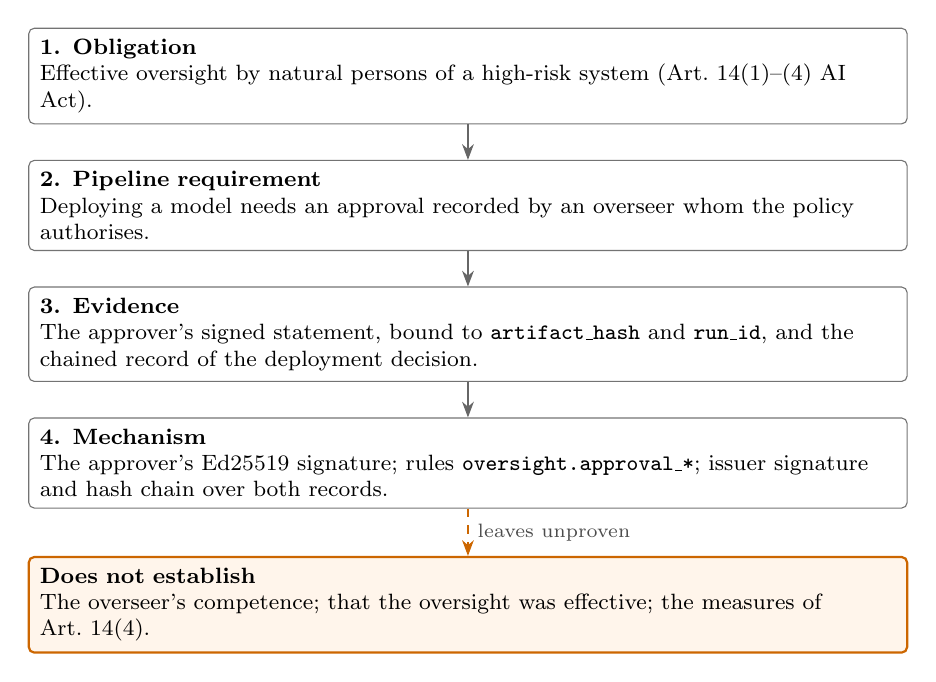
\begin{tikzpicture}[
  font=\footnotesize, node distance=4.5mm,
  stepbox/.style={draw=black!55, rounded corners=2pt, align=left, inner sep=4pt,
               text width=0.92\columnwidth-8pt},
  limit/.style={draw=orange!80!black, thick, fill=orange!8, rounded corners=2pt,
                align=left, inner sep=4pt, text width=0.92\columnwidth-8pt},
  arr/.style={-{Stealth[length=2mm]}, black!60}]
\node[stepbox] (o) {\textbf{1. Obligation}\\ Effective oversight by natural persons of a high-risk system (Art.~14(1)--(4) AI Act).};
\node[stepbox, below=of o] (r) {\textbf{2. Pipeline requirement}\\ Deploying a model needs an approval recorded by an overseer whom the policy authorises.};
\node[stepbox, below=of r] (e) {\textbf{3. Evidence}\\ The approver's signed statement, bound to \texttt{artifact\_hash} and \texttt{run\_id}, and the chained record of the deployment decision.};
\node[stepbox, below=of e] (m) {\textbf{4. Mechanism}\\ The approver's Ed25519 signature; rules \texttt{oversight.approval\_*}; issuer signature and hash chain over both records.};
\node[limit, below=6mm of m] (n) {\textbf{Does not establish}\\ The overseer's competence; that the oversight was effective; the measures of Art.~14(4).};
\draw[arr] (o) -- (r); \draw[arr] (r) -- (e); \draw[arr] (e) -- (m);
\draw[-{Stealth[length=2mm]}, orange!80!black, dashed] (m) -- node[right, font=\scriptsize, text=black!70] {leaves unproven} (n);
\end{tikzpicture}

\caption{Derivation of Art.~14 in four steps. Each step narrows the one above it, and the last box is the limit beyond which no claim built on the record may go.}
\label{fig:derivation}
\end{figure}

\subsection{The obligation-to-evidence matrix}

Table~\ref{tab:matrix} applies the derivation to the seven provisions in scope. Its last column is the one this article adds: for every row, it states what the evidence leaves unproven.

\begin{table*}[t]
\caption{Obligation-to-evidence matrix. Rule identifiers are those the Compliance Policy Engine writes in each record.}
\label{tab:matrix}
\footnotesize
\begin{tabularx}{\textwidth}{@{}>{\raggedright\arraybackslash}p{0.10\textwidth}>{\raggedright\arraybackslash}p{0.10\textwidth}>{\raggedright\arraybackslash}>{\raggedright\arraybackslash}p{0.2\textwidth}LL@{}}
\toprule
Provision & Pipeline stage & Control (\path{rule_id}) & Evidence produced & Does not establish \\
\midrule
Art. 10(2)(f)--(g) & Validation & \path{threshold.fairness} & Bias metric, threshold, decision, \path{policy_hash} & Adequacy of the metric for the population; the other duties of data governance \\
Art. 10(3) & Ingestion and training & Dataset digest recorded & \path{artifact_hash} of the dataset, \path{run_id} & Relevance, representativeness, absence of errors, completeness of the data \\
Art. 11, Annex IV & Release & Digests and off-chain references & Partial support for Annex IV, points 2(d), 2(g), 3 and 9 & Completeness of the technical documentation \\
Art. 12 & Every stage & A chained record of each event, malformed input included (\path{input.malformed}) & Signed, chained record & Events that were never emitted \\
Art. 14 & Deployment gate & \path{oversight.approval_missing}, \path{oversight.approval_invalid}, \path{oversight.approval_denied} & Signed approval and gate decision & Effectiveness and competence of the oversight; the measures of Art. 14(4) \\
Art. 15 & Validation & \path{threshold.precision} & Metric, threshold, decision & Robustness and cybersecurity; adequacy of the accuracy metric \\
Art. 72 & Monitoring & \path{monitoring.drift_alert} & Alert with indicator and threshold & Adequacy of the monitoring plan; the action taken afterwards \\
Art. 73 & Incident & \path{incident.reportable} & Incident trail: detection, report, audit query & That the deadline was met; receipt by the authority \\
Art. 78 & Export for audit & Redacted OSCAL export & Integrity anchors without sensitive fields & Absence of inference by aggregation \\
\bottomrule
\end{tabularx}
\end{table*}


Art. 12 is the only provision that every record supports, because every event is recorded, including a rejected one. The record proves what was written and never what was left unwritten, so completeness needs an external anchor (Section~6.4). Art. 14 is where a signature changes what can be proven: without it the record shows that a flag was set, and with it the record shows who approved which artefact in which run. Art. 72 is supported by an alert, which is the monitoring duty working as intended.

\subsection{Evidence model}

Every event produces one evidence record whose fields fall into five groups (Table~\ref{tab:fields}). Its JSON Schema is in Supplementary Material S1. Version 2 of the model is the one evaluated in this article. Records of version 1, the dissertation's, remain verifiable because each record declares its version and the verifier uses that version's canonical form.

\begin{table}[t]
\caption{Fields of the evidence record (version 2), by function.}
\label{tab:fields}
\footnotesize
\begin{tabularx}{\columnwidth}{@{}>{\raggedright\arraybackslash}p{0.24\columnwidth}L@{}}
\toprule
Group & Fields \\
\midrule
Identity & \path{evidence_id}, \path{run_id}, \path{scenario_id}, \path{event_type}, \path{artifact_id}, \path{artifact_type}, \path{pipeline_stage}, \path{timestamp} \\
Commitments on content & \path{payload_hash}, \path{artifact_hash}, \path{off_chain_ref} \\
Decision & \path{decision}, \path{reason}, \path{rule_id}, \path{metrics}, \path{decision_inputs}, \path{policy_id}, \path{policy_hash} \\
Normative link & \path{supports_requirements} \\
Provenance and cryptography & \path{schema_version}, \path{issuer_id}, \path{issuer_pubkey_fingerprint}, \path{sig_alg}, \path{hash_alg}, \path{parent_hash}, \path{record_hash}, \path{issuer_signature}, \path{chain_hash} \\
\bottomrule
\end{tabularx}
\end{table}


Two commitments keep the event and the artefact apart. The \path{payload_hash} is the SHA-256 digest of the event as the engine received it, and the \path{artifact_hash} is the digest of the artefact file itself (dataset, model, report), retrievable through \path{off_chain_ref} from a content-addressed store. The \path{decision_inputs} keep what the decision read beyond the metrics, including a signed approval in full, so that the decision can be re-executed from the record and the archived policy. The \path{run_id} ties together the events of one execution or release.

The canonical body is every field except \path{record_hash}, \path{issuer_signature} and \path{chain_hash}, which are derived from it (Section~5.3). Personal data in clear and the artefacts themselves never enter the record: only digests, references and metrics do. Direct identifiers in an event are replaced by keyed pseudonyms before any hash is computed (Section~5.4).

The dissertation's version 1 sealed only the event payload, under the name \path{artifact_hash}. It did not keep the decision inputs, so a decision could not be re-executed. And it could not correlate the events of one run.

\subsection{Semantics of the normative binding}

The link between a record and an article states relevance as evidence and makes no claim of compliance. It is derived from the fields the event carries: a bias metric makes the record relevant to Art. 10(2)(f), a dataset digest to Art. 10(3), any artefact digest to Art. 11, an approval to Art. 14, a drift indicator to Art. 72. Hence the field name \path{supports_requirements}: a record supports the assessment of a provision and never decides it.

The OSCAL export keeps the same distinction. Each finding targets a technical objective (\path{obj-*}), such as \path{obj-fairness-threshold} or \path{obj-drift-alert-raised}, whose status the engine can determine. The articles travel with the finding as \path{supports-requirement} properties in an \path{aia-*} namespace, and a \path{legal-assessment} property is set to \path{not-performed}.

An earlier version of the exporter shows why this distinction is a condition of correctness. It reported each finding as an article ``satisfied'' or ``not satisfied'', and drew two wrong inferences. A drift alert appeared as Art. 72 not satisfied, when the alert is Art. 72 working. A rejected malformed input appeared as Art. 12 not satisfied, when recording the rejection is Art. 12 being served. Separating the objectives a machine can assess from the articles only a lawyer can assess removed both errors.

\section{Architecture and implementation}
\label{sec:architecture}

This section describes the artefact as it was evaluated: version 2 of the evidence model, its engine, its integrity layer and its anchoring on Hyperledger Fabric. Nothing here is a target design. What was not implemented appears only as future work.

\subsection{Overview}

Six components produce and check the evidence (Figure~\ref{fig:architecture}). An event source, either the ML pipeline itself or the message bus it already uses, emits events at each stage. The Compliance Policy Engine (CPE) validates each event, decides on it and writes a signed, chained evidence record to an append-only store. Artefacts (datasets, models, reports) go to a content-addressed store and enter the record only as digests. An anchoring client commits the records, or signed batch anchors, to a Fabric network run by more than one organisation. An exporter turns the ledger into OSCAL assessment results, complete or redacted, and a verifier lets a third party check them.

The figure draws three trust boundaries. The provider runs the event source, the engine, the two stores and the issuer's signing key. The network's organisations each keep a copy of the anchors and must all endorse each transaction. The auditor receives an export and a copy of the ledger, and needs only the issuer's public key and read access to the network.

\begin{figure*}[t]
\centering
\resizebox{\textwidth}{!}{% Figure: components and trust boundaries (dashed).
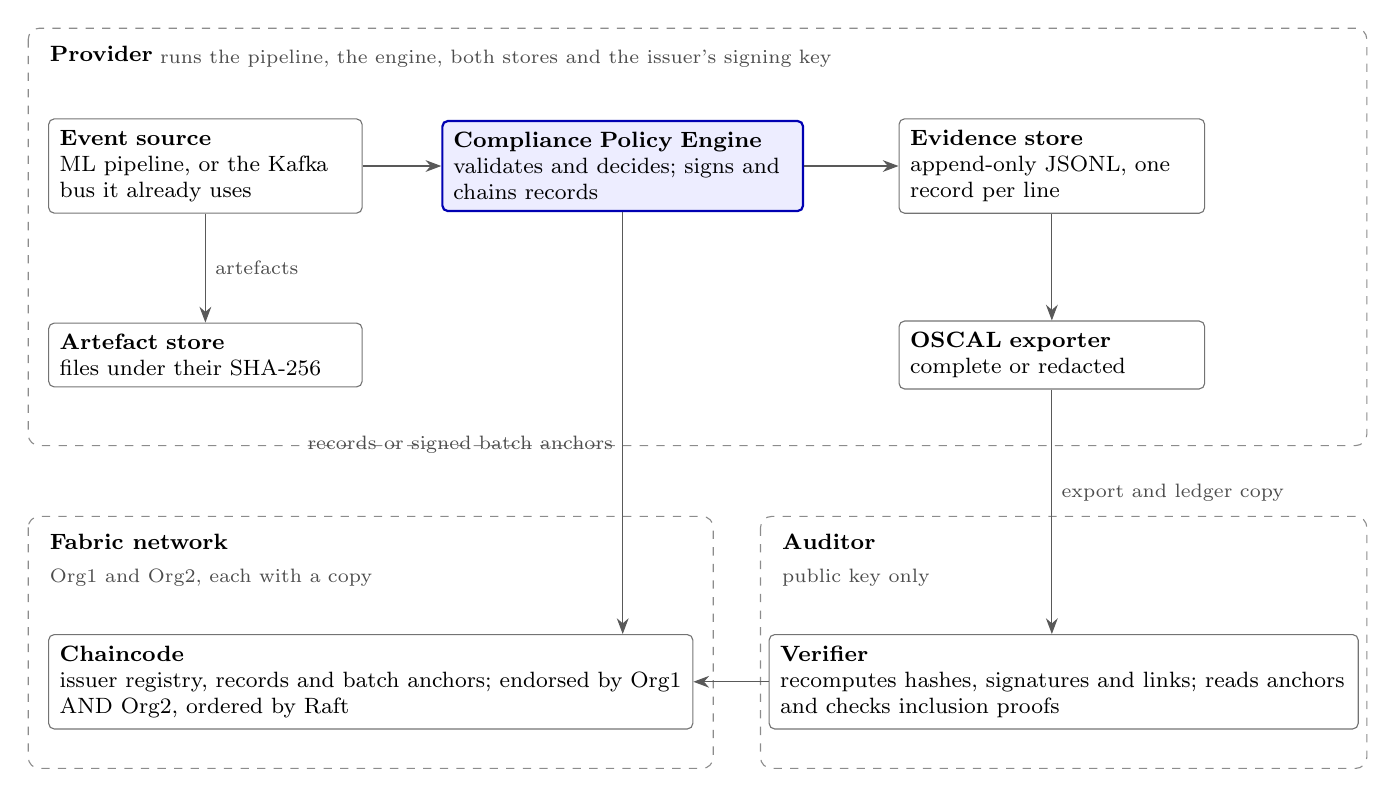
\begin{tikzpicture}[
  font=\footnotesize,
  box/.style={draw=black!55, rounded corners=2pt, align=left, inner sep=4pt, text width=#1},
  main/.style={draw=blue!70!black, thick, fill=blue!7, rounded corners=2pt, align=left, inner sep=4pt, text width=#1},
  zone/.style={draw=black!45, dashed, rounded corners=4pt},
  arr/.style={-{Stealth[length=2mm]}, black!65},
  lab/.style={font=\scriptsize, text=black!70}]
% provider zone
\draw[zone] (0,0) rectangle (17,-5.3);
\node[anchor=north west, font=\footnotesize\bfseries] at (0.15,-0.1) {Provider};
\node[anchor=north west, lab] at (1.55,-0.15) {runs the pipeline, the engine, both stores and the issuer's signing key};
\node[box=3.7cm] (src) at (2.25,-1.75) {\textbf{Event source}\\ ML pipeline, or the Kafka bus it already uses};
\node[main=4.3cm] (cpe) at (7.55,-1.75) {\textbf{Compliance Policy Engine}\\ validates and decides; signs and chains records};
\node[box=3.6cm] (ev) at (13.0,-1.75) {\textbf{Evidence store}\\ append-only JSONL, one record per line};
\node[box=3.7cm] (art) at (2.25,-4.15) {\textbf{Artefact store}\\ files under their SHA-256};
\node[box=3.6cm] (ex) at (13.0,-4.15) {\textbf{OSCAL exporter}\\ complete or redacted};
% network zone
\draw[zone] (0,-6.2) rectangle (8.7,-9.4);
\node[anchor=north west, font=\footnotesize\bfseries] at (0.15,-6.3) {Fabric network};
\node[anchor=north west, lab] at (0.15,-6.75) {Org1 and Org2, each with a copy};
\node[box=7.9cm] (cc) at (4.35,-8.3) {\textbf{Chaincode}\\ issuer registry, records and batch anchors; endorsed by Org1 AND Org2, ordered by Raft};
% auditor zone
\draw[zone] (9.3,-6.2) rectangle (17,-9.4);
\node[anchor=north west, font=\footnotesize\bfseries] at (9.45,-6.3) {Auditor};
\node[anchor=north west, lab] at (9.45,-6.75) {public key only};
\node[box=7.2cm] (vf) at (13.15,-8.3) {\textbf{Verifier}\\ recomputes hashes, signatures and links; reads anchors and checks inclusion proofs};
% connectors
\draw[arr] (src) -- (cpe);
\draw[arr] (cpe) -- (ev);
\draw[arr] (src) -- node[right, lab] {artefacts} (art);
\draw[arr] (ev) -- (ex);
\draw[arr] (cpe.south) -- node[left, lab, pos=0.55] {records or signed batch anchors} (cpe.south |- cc.north);
\draw[arr] (ex.south) -- node[right, lab, pos=0.42] {export and ledger copy} (ex.south |- vf.north);
\draw[arr] (vf.west) -- (cc.east);
\end{tikzpicture}
}
\caption{Components and trust boundaries (dashed). Only exports, ledger copies and reads of the network cross into the auditor's zone. The signing key never leaves the provider's zone.}
\label{fig:architecture}
\end{figure*}

The engine integrates without changing the pipeline. In the MultiFlow deployment it subscribes to the platform's existing Kafka topic as a consumer group of its own, and the platform's code is untouched. The bridge persists its acquisition state and any pending batch before it records them, and commits its Kafka offsets only after that state is saved, so a restart neither loses nor duplicates evidence.

Figure~\ref{fig:sequence} follows one event from emission to audit. In batched mode the engine chains records locally and anchors every $N$ records with one signed statement, and $N=1$ reduces to per-record submission.

\begin{figure*}[t]
\centering
\resizebox{\textwidth}{!}{% Figure: from pipeline event to durable evidence and audit, batched mode.
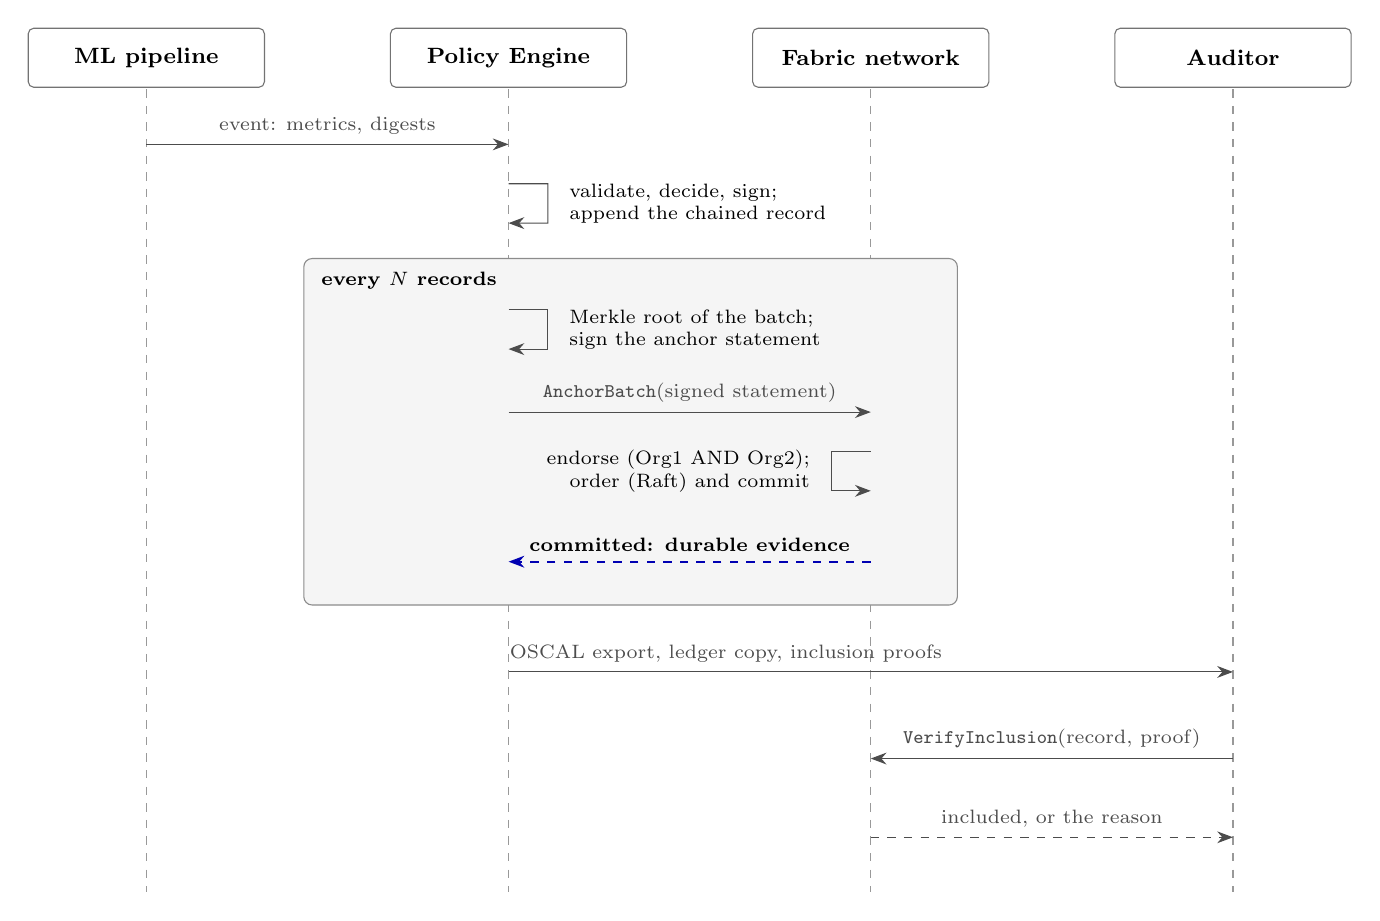
\begin{tikzpicture}[
  font=\footnotesize,
  head/.style={draw=black!55, rounded corners=2pt, minimum width=3.0cm, minimum height=0.75cm, font=\footnotesize\bfseries},
  life/.style={black!40, dashed},
  msg/.style={-{Stealth[length=2mm]}, black!70},
  ret/.style={-{Stealth[length=2mm]}, black!70, dashed},
  lab/.style={font=\scriptsize, align=center}]
\def\P{1.6} \def\E{6.2} \def\F{10.8} \def\A{15.4}
\node[head] at (\P,0) {ML pipeline};
\node[head] at (\E,0) {Policy Engine};
\node[head] at (\F,0) {Fabric network};
\node[head] at (\A,0) {Auditor};
\foreach \x in {\P,\E,\F,\A} \draw[life] (\x,-0.4) -- (\x,-10.6);
% batch frame
\fill[black!4, rounded corners=3pt] (3.6,-2.55) rectangle (11.9,-6.95);
\draw[black!45, rounded corners=3pt] (3.6,-2.55) rectangle (11.9,-6.95);
\node[anchor=north west, font=\scriptsize\bfseries] at (3.7,-2.6) {every $N$ records};
% messages
\draw[msg] (\P,-1.1) -- node[above, lab] {event: metrics, digests} (\E,-1.1);
\draw[msg] (\E,-1.6) -- ++(0.5,0) -- ++(0,-0.5) -- (\E,-2.1);
\node[anchor=west, lab, align=left] at (\E+0.65,-1.85) {validate, decide, sign;\\ append the chained record};
\draw[msg] (\E,-3.2) -- ++(0.5,0) -- ++(0,-0.5) -- (\E,-3.7);
\node[anchor=west, lab, align=left] at (\E+0.65,-3.45) {Merkle root of the batch;\\ sign the anchor statement};
\draw[msg] (\E,-4.5) -- node[above, lab] {\texttt{AnchorBatch}(signed statement)} (\F,-4.5);
\draw[msg] (\F,-5.0) -- ++(-0.5,0) -- ++(0,-0.5) -- (\F,-5.5);
\node[anchor=east, lab, align=right] at (\F-0.65,-5.25) {endorse (Org1 AND Org2);\\ order (Raft) and commit};
\draw[ret, blue!70!black, thick] (\F,-6.4) -- node[above, lab, text=black] {\textbf{committed: durable evidence}} (\E,-6.4);
\draw[msg] (\E,-7.8) -- node[above, lab, pos=0.3] {OSCAL export, ledger copy, inclusion proofs} (\A,-7.8);
\draw[msg] (\A,-8.9) -- node[above, lab] {\texttt{VerifyInclusion}(record, proof)} (\F,-8.9);
\draw[ret] (\F,-9.9) -- node[above, lab] {included, or the reason} (\A,-9.9);
\end{tikzpicture}
}
\caption{From event to audit in batched mode. A record is durable evidence once the anchor of its batch commits. Until then it is covered only by the provider's own chain. With $N=1$ the engine submits each record with \texttt{SubmitEvidence} instead of an anchor.}
\label{fig:sequence}
\end{figure*}

\subsection{Compliance Policy Engine}

The engine is a pure function of the event, the policy and the schema version: it reads no file and writes nothing, so a recorded decision can be re-executed with exactly the logic that produced it. Rules are evaluated in a fixed order, and the first that fires decides.

\begin{enumerate}[label=\arabic*., leftmargin=*, itemsep=1pt, topsep=3pt]\footnotesize
\item Input contract violated $\rightarrow$ rejected, \path{input.malformed}.
\item Serious-incident event $\rightarrow$ escalated, \path{incident.reportable}.
\item Precision below the minimum$^{*}$ $\rightarrow$ rejected, \path{threshold.precision}.
\item Parity difference above the maximum$^{*}$ $\rightarrow$ rejected, \path{threshold.fairness}.
\item Signed approval present but invalid $\rightarrow$ rejected, \path{oversight.approval_invalid}; signed approval that denies deployment $\rightarrow$ rejected, \path{oversight.approval_denied}; signed approval required but absent $\rightarrow$ rejected, \path{oversight.approval_missing}.
\item High risk without any approval $\rightarrow$ rejected, \path{oversight.approval_missing}.
\item Drift indicator above the threshold $\rightarrow$ escalated, \path{monitoring.drift_alert}.
\item Audit query $\rightarrow$ recorded, \path{audit.query_recorded}.
\item Otherwise $\rightarrow$ approved, \path{policy.all_checks_passed}.
\end{enumerate}
{\footnotesize $^{*}$ Only at the pipeline stages listed in \path{metric_threshold_stages}, where the metric is mandatory.}


Validation is fail-closed and runs before any rule. Identity fields must be non-empty text, \path{risk_level} must be present and belong to a closed set, and bounded metrics must be finite and lie in {[}0, 1{]}. All text, field names included, must consist of valid Unicode scalar values (RFC 8259, \S 8.2~\cite{rfc8259}), and metric names must stay distinct once converted to text. An event that fails is still recorded, as a rejection that supports only Art. 12.

The rule vocabulary is closed: ten identifiers, each written into the record as \path{rule_id}. A version 2 policy may restrict the precision and fairness thresholds to named stages (\path{metric_threshold_stages}), so that a monitoring batch without labels is not judged on accuracy. At those stages a missing metric leads to rejection. Policies are archived under the SHA-256 digest of their content, which the record carries as \path{policy_hash}. The \path{policy_id} is \path{pol-} followed by the digest's first twelve characters.

A signed approval is a statement naming the artefact digest, the run, the decision (approve or deny) and the time, signed with the approver's Ed25519 key over its RFC 8785 form. The policy lists the keys of authorised approvers. A statement from an unlisted key, with a bad signature, or naming another artefact or run is rejected as \path{oversight.approval_invalid}, and the record keeps the statement whole so that a third party can verify it.

The policy is evaluated off the ledger. The chaincode checks the integrity and authorship of what the engine wrote. It does not re-run the policy and cannot tell a correct decision from a wrong one.

\subsection{Integrity layer}

Each record is hashed, signed and chained over a canonical form of its body. Version 1 used the dissertation's serialisation: sorted keys, compact separators and ASCII escaping. Version 2 uses the JSON Canonicalization Scheme (JCS, RFC 8785)~\cite{rfc8785}, adopted for the article because it has standard implementations in both languages of the artefact (the Python issuer and the Go chaincode). Each record declares its version in \path{schema_version}, and the verifier rebuilds the canonical form of that version.

The \path{record_hash} is the SHA-256 digest of the canonical body. The \path{issuer_signature} is an Ed25519 signature (RFC 8032)~\cite{rfc8032} over the same bytes. The \path{chain_hash} is SHA-256(\path{parent_hash} $\Vert$ \path{record_hash}), where \path{parent_hash} is the previous record's \path{chain_hash}. Altering any field breaks the \path{record_hash}. Recomputing it without the key breaks the signature, and reordering or deleting a record breaks the links. The fields \path{schema_version}, \path{sig_alg} and \path{hash_alg} let a later version change algorithms without invalidating earlier records.

The store is append-only: one JSON line per record, with the head of the chain (last \path{chain_hash} and sequence number) in a separate file replaced atomically. Verification streams the file and needs no more memory as the ledger grows.

The verifier resolves the issuer's key by the \path{issuer_pubkey_fingerprint} the record names, among the keys it trusts. An unknown key and an invalid signature are different outcomes, reported separately. In the prototype, keys are files on disk. In production they belong in a hardware security module.

\subsection{Minimisation and pseudonymisation}

The record carries digests of the artefacts and never the artefacts themselves. Artefacts are written to a content-addressed store under \path{store/sha256/<digest>}, and the record keeps that path in \path{off_chain_ref} and the digest in \path{artifact_hash}. Anyone holding the artefact can recompute the digest. Anyone holding only the record learns nothing about the artefact beyond its declared type and identifier.

Direct identifiers are pseudonymised before any hash is computed. The engine replaces named fields (\path{subject_id}, \path{applicant_id}, \path{customer_id} and others) with an HMAC-SHA256 of their value under an organisation-scoped key, and records the organisation and key version beside the pseudonym. The key is versioned and can be rotated.

Pseudonymisation acts on field names, so an identifier placed in a free-text field passes through. Records remain linkable through \path{artifact_id} and timing patterns. And whoever holds the key can re-link each pseudonym to its subject: in the terms of Section~2.4, this is pseudonymisation and falls short of anonymisation.

\subsection{OSCAL export and selective disclosure}

The exporter maps a ledger onto an OSCAL 1.1.2 assessment-results document. Each record becomes one observation, whose UUID (version 5) is derived from the \path{evidence_id}, so that it stays the same across exports. Each decision becomes a finding that targets a technical objective (\path{obj-*}) and carries the supported articles and \path{legal-assessment}: \path{not-performed} as properties (Section~4.4). One assessment-log entry states whether the chain and the signatures verified, and whether each result was computed by the exporter or supplied to it.

A redacted mode serves the confidentiality of Art. 78. It removes the free text that can name a client, a project or a dataset: titles, descriptions, the \path{reason} and the subject identifier derived from \path{artifact_id}. It also removes \path{policy_id} and \path{policy_hash}, and puts in their place a keyed commitment, HMAC-SHA256($k$, \path{policy_hash}), where $k$ is a random 256-bit key per export that the provider keeps. It keeps everything a third party needs to tie a finding to the evidence: \path{record_hash}, \path{chain_hash}, \path{sig_alg}, the decision and the objective's status, the \path{rule_id}, the \path{aia-*} provisions, the issuer's key fingerprint and the UUIDs. Figure~\ref{fig:redaction} shows the same finding in both modes.

\begin{figure*}[t]
% Figure: one finding of the credit-scoring case, complete and redacted (abridged).
\begin{minipage}[t]{0.49\textwidth}
\centering\textbf{\footnotesize (a) Complete export}
\begin{lstlisting}[style=json]
"observation": {
  "title": "Pipeline event: german-credit",
  "description": "Compliance Policy Engine decision
    'rejected' for artifact credit-lr-v2 at stage
    validation. Reason: demographic parity diff
    0.111607 above threshold 0.1.",
  "subjects": [{"subject-uuid": "127c5e9d-..."}],
  "props": [
    {"name": "decision", "value": "rejected"},
    {"name": "issuer_pubkey_fingerprint",
     "value": "9b21fdca..."}],
  "relevant-evidence": [{"description": "...
    record_hash=601c6d47...; chain_hash=95cdc167...;
    signature_alg=Ed25519."}]},
"finding": {
  "title": "Technical objective obj-fairness-threshold:
    rejected for german-credit",
  "props": [
    {"name": "supports-requirement", "value": "aia-10-2-f"},
    {"name": "supports-requirement", "value": "aia-11"},
    {"name": "supports-requirement", "value": "aia-12"},
    {"name": "supports-requirement", "value": "aia-15"},
    {"name": "rule-id", "value": "threshold.fairness"},
    {"name": "legal-assessment", "value": "not-performed"},
    {"name": "policy-id", "value": "pol-16d3a1645858"}],
  "target": {"target-id": "obj-fairness-threshold",
    "status": {"state": "not-satisfied"}}}
\end{lstlisting}
\end{minipage}\hfill
\begin{minipage}[t]{0.49\textwidth}
\centering\textbf{\footnotesize (b) Redacted export}
\begin{lstlisting}[style=json]
"observation": {
  "title": "Pipeline event ev-e445128c-...",
  "description": "[REDACTED - AI Act Art. 78
    confidentiality]",


  "subjects": [{"subject-uuid": "ac9b13f7-..."}],
  "props": [
    {"name": "decision", "value": "rejected"},
    {"name": "issuer_pubkey_fingerprint",
     "value": "9b21fdca..."}],
  "relevant-evidence": [{"description": "...
    record_hash=601c6d47...; chain_hash=95cdc167...;
    signature_alg=Ed25519."}]},
"finding": {
  "title": "Technical objective obj-fairness-threshold:
    rejected",
  "props": [
    {"name": "supports-requirement", "value": "aia-10-2-f"},
    {"name": "supports-requirement", "value": "aia-11"},
    {"name": "supports-requirement", "value": "aia-12"},
    {"name": "supports-requirement", "value": "aia-15"},
    {"name": "rule-id", "value": "threshold.fairness"},
    {"name": "legal-assessment", "value": "not-performed"},
    {"name": "policy-commitment", "value": "91e1b250..."}],
  "target": {"target-id": "obj-fairness-threshold",
    "status": {"state": "not-satisfied"}}}
\end{lstlisting}
\end{minipage}

\caption{One finding of the credit-scoring case, record 8 (validation of model v2, rejected at the fairness gate), in the complete and the redacted export; abridged. Exported from the run's ledger with the exporter described here.}
\label{fig:redaction}
\end{figure*}

Redaction has to account for identifiers that can be derived. An earlier version computed the redacted subject's UUID from the \path{artifact_id} over a public namespace. Anyone holding a candidate identifier could recompute the UUID and confirm the match, so the identifier left the text but stayed confirmable from the document. The redacted subject is now derived from the \path{payload_hash}, a digest already present in the record that cannot be recomputed without the whole event.

The policy raised the same problem in a stronger form. The first version of the redacted export kept the plain \path{policy_hash}, and a policy has few unknowns: a handful of thresholds on a coarse scale, a list of stages and a flag. Someone who knows the policy format, which is public, and the approver entry can hash every candidate policy and compare. Over a grid of 356,400 candidates, this search recovered every threshold of the credit-scoring policy from the digest, after 242,335 candidates (Section~6.7). The \path{policy_id} that export removed was the digest's prefix, so removing it withheld nothing. The keyed commitment closes both channels. Within one export the same policy gives the same value, so a change of policy stays visible, and a party given $k$ with the policy, or with its digest, can check the commitment.

With the redacted document alone, a third party can compare its anchors against a copy of the ledger or against the anchors on the network. Recomputing them requires the records. Redaction limits what the export discloses. It does not reach the network, where with per-record anchoring every organisation reads the full records, reasons and metrics included. Nor does it limit what an authority may demand: a market surveillance authority may still request documentation and data under Art. 74(12)--(13), and a notified body under Annex VII, points 4.3 and 4.4.

\subsection{Ledger anchoring on Hyperledger Fabric}

The chaincode checks integrity and authorship, and records who submitted what. It exposes eight functions: \path{RegisterIssuer}, \path{SubmitEvidence}, \path{AnchorBatch}, \path{VerifyChain}, \path{VerifyInclusion}, \path{QueryByRequirement}, \path{GetEvidence} and \path{GetAnchors}.

Issuer keys are governed on chain. Only the organisation acting as compliance authority may register an issuer's Ed25519 key, stored under its fingerprint. On every submission the chaincode fetches the key by the fingerprint the record names, never from the caller, verifies the signature over the record's canonical body, recomputes \path{record_hash} and \path{chain_hash}, and checks that \path{parent_hash} equals the current head. It then stamps the submitting organisation's MSP identifier and the submitter's identity beside the record. Reading and writing a single head pointer makes Fabric's multi-version concurrency control serialise concurrent submissions, so the chaincode imposes one order.

The endorsement policy, \path{AND('Org1MSP.peer','Org2MSP.peer')}, requires a peer of each organisation to endorse every transaction, so neither organisation can change the ledger's state alone. Integrity then has two layers: the application's chain of records and the orderer's chain of blocks. The two signatures are also distinct: the issuer's Ed25519 signature proves who produced a record, and the X.509 identity of Fabric proves who submitted it.

In batched mode the engine chains records locally and, every $N$ records, anchors one signed statement instead of $N$ records. The statement names the stream, the first and last sequence numbers, the Merkle root over the batch's \path{record_hash} values (RFC 9162 tree, with distinct prefixes for leaves and nodes) and the \path{chain_hash} of the batch's last record. The issuer signs its RFC 8785 form. \path{AnchorBatch} checks the signature against the registry and that the batch follows the previous one of its stream. \path{VerifyInclusion} takes a record and the inclusion proof the issuer hands out, and checks without writing that the record verifies, that the same issuer signed the anchor, and that the proof leads from the \path{record_hash} at the claimed position to the anchored root. The proof grows with $\log_2 N$, and the records themselves stay with the provider. $N=1$ reduces to per-record submission, kept for comparison (Section~6.6).

Endorsement leaves the choice of policy to the provider. The \path{policy_hash} in each record makes a change of policy observable to every organisation, but nothing on the ledger authorises the change: a provider can switch policies, and the ledger only shows that it did.

\subsection{Threat model and trust assumptions}

We consider five adversaries:

\begin{itemize}
\tightlist
\item
  an outsider with read access to exports or ledger copies;
\item
  an insider who can edit the stored ledger but does not hold the issuer's key;
\item
  an insider who holds the issuer's key;
\item
  a single organisation of the Fabric network acting alone;
\item
  a compromised producer of events, upstream of the engine.
\end{itemize}

The artefact's guarantees rest on three assumptions: the engine's code is the code that was reviewed, the issuer's key is held only by the engine, and the event source's clock is correct. Under them, the records establish what the engine decided and when it recorded it. Whether the event it received was true lies outside them.

The architecture therefore moves trust from the record, which a third party can now check, to the component that decides what is recorded. Which of the five adversaries each configuration detects is a measured result, reported once, in Section~6.4 (Table~\ref{tab:tamper}).

\section{Evaluation}
\label{sec:evaluation}

The evaluation answers the three research questions with measurements whose protocols were committed before they ran. Every number below comes from a JSON file in the public repository and is given with the environment it was measured in.

\subsection{Setup}

Two environments were used, and timings come only from the second.

\begin{table*}[t]
\caption{Environments. Timings come only from the physical machine.}
\label{tab:env}
\footnotesize
\begin{tabularx}{\textwidth}{@{}>{\raggedright\arraybackslash}p{0.2\textwidth}LL@{}}
\toprule
Environment & Hardware and software & Used for \\
\midrule
Cloud container & Linux x86\_64; Python 3.13; scikit-learn 1.9.1; Go 1.24.7 & Functional correctness, the credit-scoring case, regeneration of the dissertation's runs, tamper attacks in A--B+, answerability; no timing is reported from it \\
Physical machine & Apple M4 Pro (14 cores), 24\,GB; macOS 26.6.2; Python 3.12.7; APFS & Cost ablation (Section~6.5) \\
Same machine, Docker Desktop 29.8.0 (14 CPUs, 8\,GB) & Hyperledger Fabric 2.5.10 (arm64 images); two organisations, one CA each, one Raft orderer; LevelDB, and CouchDB 3.4.2 for a query run & Anchoring (Section~6.6), configuration C of the tamper experiment, audit question Q12 \\
\bottomrule
\end{tabularx}
\end{table*}


The data are the six canonical scenarios and a three-event serious-incident sequence; the Statlog German Credit dataset (1,000 applicants)~\cite{hofmann1994} for the credit-scoring case; and two streams of the MultiFlow industrial platform~\cite{torres2026}: Muvu (29 events) and Steel\_Industry (35,040 readings, 1,750 events). Protocols, results and figure scripts are archived with a DOI~\cite{artefacts} (see the data availability statement).

\subsection{Functional correctness}

The engine reproduces the dissertation's decisions under the version 2 evidence model. The six canonical scenarios yield one approval, three rejections (precision, fairness, missing approval), one escalation for drift and one recorded audit query, each under the same rule as in version 1. The incident sequence yields two escalations under \path{incident.reportable} and one recorded query, all three supporting Art. 73. Re-executing every decision from its record and the archived policy returns the same decision and \path{rule_id} for all 1,788 regenerated records and all 16 records of the credit case.

The input boundary is pinned by a matrix of 24 malformed or edge-case events: the dissertation's 16, plus 8 for the version 2 fields and the numeric domain of RFC 8785. Each case gets the same outcome in the Python issuer and the Go chaincode. The dissertation's sensitivity analysis over 45 threshold combinations still applies to the decision logic, which version 2 left unchanged: approvals range from 0/6 to 4/6, and the decision profile is stable to $\pm$6.25 \% of the precision threshold. The grids for fairness and drift are too coarse to claim fine stability for those thresholds.

\subsection{Real-data cases}

Table~\ref{tab:runs} summarises the five runs. Every chain verifies and every decision re-executes.

\begin{table*}[t]
\caption{Decisions and verification per run (schema version 2).}
\label{tab:runs}
\footnotesize
\begin{tabularx}{\textwidth}{@{}Lrrrrrrr@{}}
\toprule
Run & Events & Approved & Rejected & Escalated & Recorded & Chain & Re-execution \\
\midrule
Canonical scenarios & 6 & 1 & 3 & 1 & 1 & 6/6 & 6/6 \\
Incident sequence (Art. 73) & 3 & 0 & 0 & 2 & 1 & 3/3 & 3/3 \\
Credit scoring, German Credit & 16 & 11 & 4 & 1 & 0 & 16/16 & 16/16 \\
MultiFlow, Muvu (replay) & 29 & 12 & 0 & 17 & 0 & 29/29 & 29/29 \\
MultiFlow, Steel\_Industry (replay) & 1,750 & 94 & 0 & 1,656 & 0 & 1,750/1,750 & 1,750/1,750 \\
\bottomrule
\end{tabularx}
\end{table*}


\textbf{Credit scoring.} The pipeline emits a record at every stage, each run under its own \path{run_id}: ingestion and split of the dataset, training, validation and, for the second model, two deployment requests and six monitoring batches. The protected attribute (age, under 25 against 25 and over, as in AI Fairness 360~\cite{bellamy2019}) and every threshold were fixed before training. The minimum precision, 0.68, was calibrated on a pilot partition that was then discarded. On the validation set, the unmitigated model reaches precision 0.793 and the model trained with reweighing~\cite{kamiran2012} 0.800, but both show a demographic parity difference of 0.112, above the maximum of 0.10. Both validations are therefore rejected under \path{threshold.fairness}, and so are both deployment requests, before the approval rule is reached. This holds whether or not the request carries a valid signed approval.

Monitoring follows the second model on six batches of 50 test cases, with a subgroup over-sampled at a share rising from 0.30 to 0.95. The Population Stability Index~\cite{siddiqi2006} of the scores rises from 0.042 to 0.930 and crosses the threshold of 0.25 only in the last batch, which escalates under \path{monitoring.drift_alert}. The acceptance checks all pass. The 10 metrics in the ledger are recomputed, identically, from the artefacts in the store, and all 16 artefact digests are recomputed from their \path{off_chain_ref}.

A post hoc analysis over 500 partitions shows how much of this outcome is one draw. The reweighed model passes validation in 44 \% of partitions (95 \% interval 40--48 \%) and the unmitigated one in 26 \% (23--30 \%). The decision taken on the validation set agrees with the one the test set would give in only 49 \% and 58 \% of partitions. The evidence records exactly what was decided and on which numbers. The stability of the estimate behind the decision is another matter (Section~7.1).

\textbf{MultiFlow.} The two industrial streams were regenerated under version 2 by replaying the platform's CSV files through the bridge's own logic, without Kafka. Batch by batch, the replay reproduces the dissertation's live runs: the same decision and the same reason, drift score included, for 29 of 29 and 1,750 of 1,750 batches. Only the observational half of the policy is exercised. Precision and parity come from the observer's configuration (0.85 and 0.03), and the approval flag is an assumption, so the escalations measure drift and nothing else.

\subsection{Tamper evidence}

Table~\ref{tab:tamper} gives the observed outcome of each attack on the credit-scoring ledger (16 records; the attacked record is the eighth). In B+ the signed head is published every five records, and in C every record is anchored on the Fabric network. All 48 cells of A--B+ and all nine attacks in C came out as the protocol expected.

\begin{table*}[t]
\caption{Attacks detected by a third party's check, per configuration (observed). In B+ the signed head is published every five records; in C every record is anchored on the Fabric network.}
\label{tab:tamper}
\footnotesize
\begin{tabularx}{\textwidth}{@{}Lccccc@{}}
\toprule
Attack & A & B0 & B & B+ & C \\
\midrule
T1 Alter a field of an intermediate record & no & yes & yes & yes & yes \\
T2 Alter only the signature & -- & -- & yes & yes & yes \\
T3 Alter and recompute every hash, without the key & no & no & yes & yes & yes \\
T4 Swap two records & no & yes & yes & yes & yes \\
T5 Delete an intermediate record & no & yes & yes & yes & yes \\
T6a Truncate a suffix that crosses an anchor & no & no & no & yes & yes \\
T6b Truncate a suffix after the last anchor & no & no & no & no & yes$^{a}$ \\
T7a Rewrite with the issuer's key, crossing an anchor & no & no & no & yes & yes \\
T7b Rewrite with the issuer's key, after the last anchor & no & no & no & no & yes$^{a}$ \\
T8 Omit an event at the source & no & no & no & no & --$^{b}$ \\
T9a Inject a forged event upstream & no & no & no & no & --$^{b}$ \\
T9b Inject a forged approval upstream & no$^{c}$ & no$^{c}$ & no$^{c}$ & no$^{c}$ & --$^{b}$ \\
\bottomrule
\end{tabularx}

\smallskip
\raggedright\footnotesize
$^{a}$ The same records are altered as in B+; in C they are anchored, so no unanchored suffix exists.
$^{b}$ These attacks act before anything reaches a ledger and were not repeated for C.
$^{c}$ The record is well formed and passes the check, but the engine rejects the forged approval at the gate (\path{oversight.approval_invalid}) in every configuration.
-- under A and B0 for T2: no signature to alter.
\end{table*}



T3 measures what the signature adds to the hash chain: without the key, a consistent rewrite of the hashes passes B0 and fails B. T6 and T7 measure what an external anchor adds to a signed log. Truncation and a rewrite by a key holder become detectable, but only up to the last anchor, and anchoring every record on the network closes that window. T8 and T9a are outside the reach of every configuration, because the evidence can only attest what the engine was given. T9b, the one upstream forgery that is caught, is stopped by the engine's check of the approver's signature before anything is stored.

\subsection{Cost of verifiable evidence}

Signing costs little. Table~\ref{tab:cost} gives the latency per event of each arm of the ablation, measured on the physical machine in ten rounds of 200 events after 50 discarded, with the order of the arms rotated by a Williams design.

\begin{table*}[t]
\caption{Latency per event (ms) on the physical machine: median of round medians [IQR over 2,000 events] and 95th percentile. W1: the dissertation's approved validation event; W2: the six canonical scenarios in turn.}
\label{tab:cost}
\footnotesize
\begin{tabularx}{\textwidth}{@{}Lcccc@{}}
\toprule
Arm or paired difference & W1 median [IQR] & W1 P95 & W2 median [IQR] & W2 P95 \\
\midrule
A, SQLite row & 0.26 [0.24 to 0.31] & 0.50 & 0.29 [0.26 to 0.32] & 0.45 \\
B0, hash chain & 0.31 [0.29 to 0.35] & 0.44 & 0.33 [0.30 to 0.37] & 0.52 \\
B, signed & 0.33 [0.30 to 0.37] & 0.48 & 0.34 [0.31 to 0.39] & 0.52 \\
B+, anchored every 100 events & 0.34 [0.31 to 0.38] & 0.46 & 0.35 [0.32 to 0.40] & 0.52 \\
\midrule
B0 $-$ A: canonical form, hashing, append-only file & 0.048 [0.0015 to 0.082] & 0.14 & 0.045 [0.011 to 0.079] & 0.15 \\
B $-$ B0: Ed25519 signature & 0.017 [$-$0.016 to 0.053] & 0.11 & 0.016 [$-$0.019 to 0.052] & 0.12 \\
B $-$ A: verifiable log against a database row & 0.068 [0.022 to 0.098] & 0.16 & 0.059 [0.026 to 0.096] & 0.16 \\
B+ $-$ B: anchoring & 0.0069 [$-$0.027 to 0.039] & 0.099 & 0.0088 [$-$0.027 to 0.043] & 0.12 \\
\bottomrule
\end{tabularx}
\end{table*}


An event takes about 0.3 ms in every arm, the engine's decision included, which all arms share. A verifiable centralised log adds 0.068 ms per event to a plain database row (W1), and the Ed25519 signature accounts for 0.017 ms of that. Anchoring falls on one event in a hundred: the anchor operation itself takes 0.080 ms, and its amortised cost (the mean of B+ $-$ B, $-$0.001 ms) cannot be told apart from zero. On macOS, \path{fsync} does not force the drive's write cache, for the append-only file or for SQLite, so both arms are treated alike.

The cost does not grow with the ledger (Figure~\ref{fig:growth}). Over 10,000 records, the median per block of 1,000 moves from 0.31 to 0.32 ms for B and from 0.27 to 0.26 ms for A, and every arm's ledger verifies at the end. The dissertation's prototype rewrote the whole ledger file on each event, so its latency grew with the ledger. Append-only persistence removed that growth.

\begin{figure}[t]
\centering
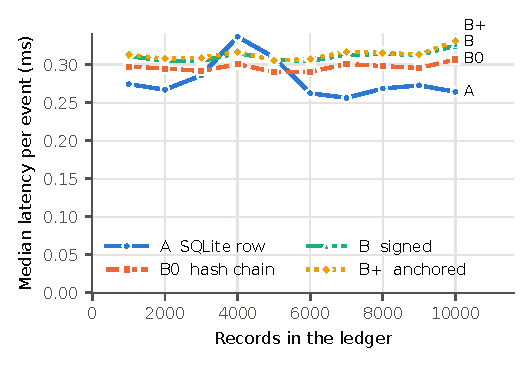
\includegraphics[width=\columnwidth]{figures/F4_latency_vs_ledger_size.pdf}
\caption{Median latency per event against the number of records in the ledger, per arm, in blocks of 1,000 events (W1).}
\label{fig:growth}
\end{figure}

Set against the event cadence of the two real cases, the cost is negligible. At the rate of the live MultiFlow run (21.7 events/s, Section~6.6), a verifiable log adds about 1.5 ms of work per second of stream. The credit-scoring pipeline emits only 16 records over two training runs.

\subsection{Cost of ledger anchoring}

The cost of the ledger lies in ordering. With one transaction in flight, the orderer cuts each block only when its BatchTimeout expires, so every anchoring transaction waits for it, whatever $N$. The latency to durable evidence is 2,028 ms with the 2 s timeout and 278 ms with 250 ms, about 28 ms above the timeout, and it barely moves up to $N=500$ (2,039 and 289 ms; Figure~\ref{fig:anchoring}b). At $N=1$ the network makes 0.49 records durable per second, which reproduces the dissertation's figure of about 0.5.

Throughput therefore grows in proportion to $N$ (Figure~\ref{fig:anchoring}a): from 0.49 to 245 records per second with 2 s, and from 3.6 to 1,730 with 250 ms. An anchor for 500 records is one transaction carrying one Merkle root, so the number of records no longer reaches the network. Backfilling the 1,750 events of the Steel\_Industry stream would take about an hour at $N=1$ with the default timeout, and about one second at $N=500$ with 250 ms.

The price of batching is the wait for a batch to fill. At the event rate of the live MultiFlow run, 21.7 events per second, per-record anchoring cannot keep up with either timeout, and neither can $N=10$ with 2 s: the queue would grow without bound. Where anchoring keeps up, the expected time from emission to durable evidence is the measured anchor latency plus the mean wait to fill the batch, $(N-1)/(2\lambda)$ (Figure~\ref{fig:anchoring}c). It is 0.48 s at $N=10$ with 250 ms, 3.2 s at $N=50$ with 2 s, and 11.8 to 13.6 s at $N=500$. A provider thus chooses $N$ and the timeout from its event rate and from how long a record may stay covered only by its own chain.

\begin{figure*}[t]
\centering
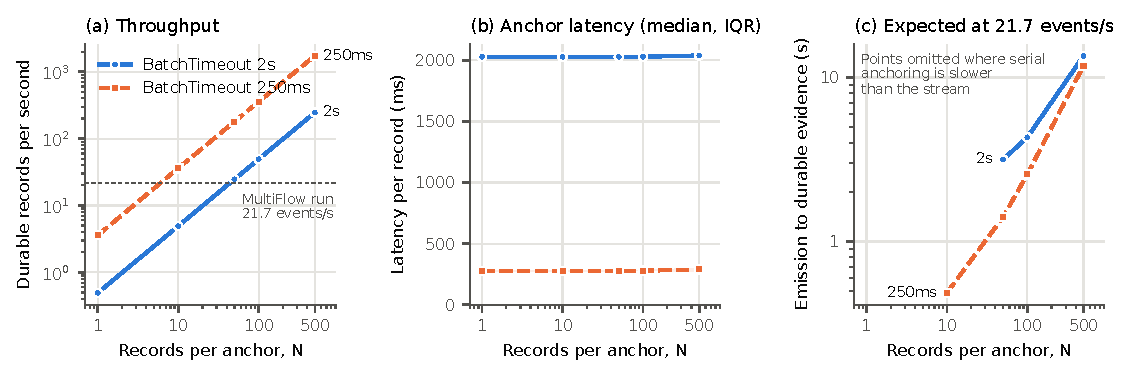
\includegraphics[width=\textwidth]{figures/F5_anchoring_vs_batch_size.pdf}
\caption{Anchoring on the Fabric network against records per anchor, $N$. (a) Durable-evidence throughput, with the event rate of the live MultiFlow run as a reference line. (b) Measured latency per record (median and IQR). (c) Expected time from emission to durable evidence at that rate: the measured latency plus the analytic wait to fill the batch. Points where serial anchoring is slower than the stream are omitted.}
\label{fig:anchoring}
\end{figure*}

Verification is cheap and independent of $N$. \path{VerifyInclusion} takes 1.6 ms (median; 95th percentile 2.3 to 3.1 ms) on both state databases, and an inclusion proof grows with $\log_2 N$, from 337 bytes at $N=10$ to 673 at $N=500$. \path{VerifyChain} over the per-record chain takes 206 ms for 601 records on LevelDB (0.34 ms per record) and 102 ms for 201 records on CouchDB (0.51 ms per record). The CouchDB network held one repetition of the chain against three on LevelDB, so only the per-record figures compare. The first call of each query paid a warm-up of several seconds, which raises the 95th percentile of \path{VerifyChain} in the 2 s run to 438 ms.

The endorsement policy held. An anchor endorsed by Org1 alone was refused at validation with \path{ENDORSEMENT_POLICY_FAILURE} on all three networks. The transaction stays in its block, marked invalid, and the world state did not change.

\subsection{Auditability}

Table~\ref{tab:audit} condenses the answers to the fourteen audit questions of Section~3 in four configurations. In C, the network is represented by a signed log anchored after every record, as the Fabric run provides, and Q12 is answered from the Fabric run itself. The full matrix is in the supplementary material.

\begin{table}[t]
\caption{Audit questions per configuration: number asked (Q), answerable yes / partial / no (Y/P/N), and answers verifiable by a third party (V). Q14, a check that the redacted export discloses nothing it should withhold, applies only to D.}
\label{tab:audit}
\footnotesize
\begin{tabularx}{\columnwidth}{@{}Lccc@{}}
\toprule
Configuration & Q & Y/P/N & V \\
\midrule
A, plain SQLite log & 13 & 3/2/8 & 0 \\
B, signed log, policy archive, artefact store & 13 & 10/2/1 & 6 (+6 in part) \\
C, B anchored on the ledger, complete OSCAL export & 13 & 13/0/0 & 13 \\
D, redacted OSCAL export only & 14 & 3/5/6 & 0 \\
\bottomrule
\end{tabularx}
\end{table}


Q14, a check that the redacted export discloses nothing it should withhold, applies only to D.

C answers every question, and every answer can be checked without trusting the provider. The chaincode stamps the submitting organisation on each anchor, which answers Q12 (Org1MSP for all 16 records). Q2, who approved the deployment, is answerable only where approvals are signed, while A holds a Boolean flag. Q6, whether re-execution reproduces a decision, needs the decision inputs and the policy archive, which only B and C keep. Q11, whether the sequence is complete between two dates, is answerable only in C, because a signed log cannot show that nothing was cut after its last record.

The redacted export answers less, by design. From D alone, Q13 (which articles are supported, with which technical outcome) is answerable but not verifiable, since the export carries anchors and no record bodies. For Q14, none of the 60 items checked appears in the redacted export: artefact names and digests, the subject identifiers derived from them, reasons, metric values, scenario names, and the policy's threshold fields and values. The search of Section~5.5 tried all 356,400 candidate policies against the policy commitment and recovered nothing. The same search on the first version of the export, which carried the plain digest, recovered the policy. With the provider's key, the commitment opened against the archived policy.

\subsection{Interoperability and conformance}
\label{sec:eval-interop}

The evidence crosses three implementations with the same bytes. Every OSCAL export validates against the NIST schema: the complete and redacted exports of the credit case and of the four regenerated runs, and the dissertation's 18 published exports. The Python issuer and the Go chaincode agree on 6 of 6 canonicalisation vectors of version 1 and 4 of 4 of RFC 8785, on the 24 boundary cases, and on the Merkle roots, inclusion proofs and signed anchors of the batched mode. The browser-based Ledger Explorer recomputes the hash of every record of the version 1 and version 2 ledgers.

That agreement was not there at first. Table~\ref{tab:defects} lists the eight defects that appeared between the Python issuer and the Go chaincode, during the dissertation and its later review.

\begin{table*}[t]
\caption{Defects between the Python issuer and the Go chaincode, and their corrections.}
\label{tab:defects}
\footnotesize
\begin{tabularx}{\textwidth}{@{}>{\raggedright\arraybackslash}p{0.16\textwidth}>{\raggedright\arraybackslash}p{0.2\textwidth}LL@{}}
\toprule
Defect & Symptom & Cause & Correction \\
\midrule
HTML and non-ASCII escaping & \path{record_hash} differs between issuer and chaincode & Go's encoder escapes HTML characters and keeps non-ASCII literal; Python's default does the opposite & One canonical form specified on bytes; RFC 8785 in version 2 \\
Fingerprint taken for the key & Every Ed25519 verification fails & The key's SHA-256 fingerprint used as verification material & Key resolved from a registry by its fingerprint \\
Range-read order & Chain reconstruction breaks & Fabric range reads order keys lexicographically, not by insertion & Zero-padded sequence keys \\
\path{0.0} rewritten as \path{0} & Digest diverges by one byte & A float64 round trip in Go drops the issuer's literal & Original number literals kept (\path{json.RawMessage}) \\
Null optional field & A record that verifies at the source fails at the destination & Go decodes null into an empty string & Optional field as a pointer \\
New fields dropped & No record of the new format verifies & \path{encoding/json} silently discards fields the struct does not declare & In version 2, the hash is computed over the record's own members \\
Lone Unicode surrogate & A body signed and verified in Python diverges in Go & Such strings are outside interoperable JSON (RFC 8259, \S8.2) & Input domain restricted to Unicode scalar values \\
Colliding non-text keys & Two different malformed inputs get the same payload digest & An integer key renders like the string of its digits & Normalisation falls back to an ordered list of pairs on collision \\
\bottomrule
\end{tabularx}
\end{table*}


A canonical form must therefore be specified on bytes, independently of any one language's data model, and a shared boundary matrix works as a conformance test between implementations.

\section{Discussion}
\label{sec:discussion}

The results support the thesis in its three parts: the obligations can be turned into evidence a third party can verify, the cryptography that makes it verifiable costs little, and what costs is distributed ordering.

\subsection{What the evidence proves, and what it does not}
\label{sec:disc-proves}

The evidence proves the integrity and provenance of what the engine recorded, and the link of each decision to its rule, its policy and the provisions it supports. Table~\ref{tab:tamper} marks the boundary. Any alteration of a record after issuance is detected by a third party holding the issuer's public key (T1--T5), and truncation or rewriting by a key holder is detected up to the last anchor (T6, T7). Because every decision re-executes from its record and the archived policy (Section~6.2), a reader can check not only that a record is intact but that the recorded decision follows from the recorded inputs.

What the evidence does not prove is as precise. It does not prove that the metrics were true at the source, that no event was withheld (T8), or that an event came from the producer it names (T9a). The one exception is the signed approval, whose author and authorisation the engine verifies (T9b). Nor does the evidence make the decision behind it reliable. In the credit case the fairness gate rejected both models on one partition, while across 500 partitions the reweighed model would have passed in 44\,\% of them, and the validation decision matched the test decision in only about half (Section~6.3). The record states exactly what was decided and on which numbers. The policy compares point estimates with thresholds and does not express their uncertainty.

Trust thus comes to rest on the engine that decides what is recorded and on the source that feeds it. Reproducible builds of the engine and attested execution in trusted execution environments are the routes to reduce that trust, and are left to future work.

\subsection{When is a ledger warranted?}
\label{sec:disc-ledger}

Table~\ref{tab:tamper} and Figure~\ref{fig:anchoring} together answer the question with costs. A signed log (B) gives evidence of mutation for 0.068\,ms per event. Publishing its signed head (B+) closes truncation and rewriting by a key holder up to the last anchor, for an anchor operation of 0.080\,ms every hundred events. What matters for B+ is where the head goes: it must be published where the provider cannot retract it, such as a transparency log, an RFC 3161 time-stamping authority~\cite{rfc3161} or an endpoint run by the supervisor.

A permissioned ledger (C) adds three properties that neither provides. No organisation can change the ledger's state alone, as the refused single-organisation anchor showed. Every anchor names the organisation that submitted it, which answers Q12. And each organisation keeps its own copy of the history. Its price is ordering: about one BatchTimeout per transaction, which batching turns from a throughput limit into a delay of seconds at the cadences we observed.

As a rule of thumb, a single organisation audited by an external authority may find B+ sufficient, provided the anchors go to a party the authority trusts. Settings with several parties, such as provider and deployer, a notified body, a supply chain or a sector consortium, are where C earns its cost, with batches sized to the event rate. One property of C was not measured: the administrative independence of its organisations, since both ran on the same machine.

\subsection{Legal significance}
\label{sec:disc-legal}

Three bodies of law give the evidence a role beyond supervision. We state each as of November 2026.

\paragraph{Electronic ledgers under eIDAS} Under Art.~45k(1) of Regulation (EU) No 910/2014, as amended~\cite{eidas_2024}, an electronic ledger cannot be denied legal effect or admissibility as evidence solely because it is electronic or because it does not meet the requirements for qualified ledgers. The artefact falls under that paragraph: it is a sequence of electronic records that ensures their integrity and the accuracy of their chronological ordering. The presumption of Art.~45k(2), of unique and accurate sequential ordering and of integrity, attaches only to qualified electronic ledgers, which this is not. Qualification would require a qualified trust service provider (Art.~3(53)). Compliance with ETSI EN 319 401 and, for a service built on distributed ledger technology, ISO 23257:2022 and ISO/TS 23635:2022 gives a presumption of conformity with the requirements for qualified electronic ledgers (Art.~45l(2))~\cite{qel_2025,alamillo2024}. Admissibility leaves the weight of the evidence to the court, and no court or authority has assessed it.

\paragraph{Product liability} Directive (EU) 2024/2853~\cite{pld_2024} applies to products, software included, placed on the market or put into service after 8 December 2026, a year before the Annex III requirements of the AI Act. Its Art.~9(1) lets a court order the defendant to disclose relevant evidence at its disposal, and Art.~10(2)(a) presumes the product defective if the defendant fails to do so. Art.~9(4) and (5) direct the court to protect trade secrets and confidential information while it orders disclosure. Selective disclosure (Section~5.5) is an instrument for that duty, prepared before any litigation: the redacted export lets the other party and the court check that findings map to provisions and that anchors match, without reading the policy logic. The provider can later open the policy commitment to the court alone, by disclosing its key with the policy.

The directive is asymmetric. Failure to comply with mandatory safety requirements supports a presumption of defectiveness (Art.~10(2)(b)) and is one of the circumstances of the assessment (Art.~7(2)(f)). Compliance does not prove the absence of a defect, because defectiveness is assessed on all the circumstances. Verifiable evidence that the pipeline ran its checks therefore weighs in the assessment without closing it. Art.~10(4) requires the court to presume defectiveness, causation or both where, despite disclosure, the claimant faces excessive difficulties, in particular because of technical or scientific complexity, and shows that they are likely. Art.~10(5) lets the defendant rebut the presumption. A verifiable record lowers the asymmetry of information on which both parties rely, without taking either side.

\paragraph{Technical documentation} The artefact supports parts of Annex~IV, points 2(d), 2(g), 3 and 9, with records and digests that the pipeline produces as it runs. The rest of the technical documentation still needs human preparation. The full mapping is in the supplementary material.

\subsection{Implications for standards}
\label{sec:disc-standards}

\paragraph{OSCAL} NIST publishes no OSCAL catalogue for the AI Act. Our export suggests how one should be modelled: technical objectives, which a machine can assess, kept apart from legal provisions, which it cannot (Section~4.4). A public catalogue of controls for the AI Act, with the technical objectives as its parts, is the natural next step.

\paragraph{Canonical JSON} The eight defects of Table~\ref{tab:defects} show that a canonical form specified on one language's data model breaks between implementations. Adopting RFC 8785 removed the encoding defects. The remaining ones were boundary cases, such as nulls, lone surrogates, key types and number literals, that only a shared conformance matrix exposed. Standards that rely on signed JSON should ship such a matrix with the canonical form.

\paragraph{Logging standards} prEN ISO/IEC 24970 on AI system logging closed its formal vote in October 2026 and had not been published as of November 2026~\cite{iso24970}. The fields of the evidence model should be aligned with it once it is published.

\subsection{Adoption path}
\label{sec:disc-adoption}

Adoption can be incremental. A provider can start with the evidence model and the engine, which add 0.068\,ms per event to its pipeline. It can then publish its signed head to an external party when an authority or a contract asks for completeness, and move to a permissioned ledger when several parties must share the history. Three prerequisites hold at every step: a pipeline mature enough to emit events at each stage, since the engine consumes events and does not create them; custody of the signing key in a hardware security module; and separation of duties between those who run the engine and those who hold its key.

\section{Threats to validity}
\label{sec:threats}

We follow the usual classification of threats~\cite{wohlin2012}.

\paragraph{Internal validity} The authors designed the artefact and evaluated it. Three measures limit the bias this invites: every protocol, with its parameters and expected outcomes, was committed to the public repository before the measurement it governs; every acceptance criterion is checked by an automated assertion; and every result file is public. Two deviations are reported as such. The first cost run and the first anchoring run at 2\,s ran beside unrelated containers. Both were repeated with nothing else running, and the first files are kept and marked as superseded. A review of the manuscript found that the redacted export kept a policy digest from which the thresholds could be recovered. The exporter was changed and the audit questions were run again under an amendment recorded beforehand. The first of these runs matched a metric value inside a timestamp and was repeated, and its files are also kept as superseded. The analysis of stability across 500 partitions was decided after the main run and is reported as post hoc.

\paragraph{External validity} The evaluation covers one regulated domain, credit scoring, and one industrial stream, and the drift in the credit case was induced. The Fabric network is a laboratory network: two organisations on one machine, one Raft orderer, no TLS between chaincode and peer, and demonstration keys. All timings come from one machine, an Apple M4 Pro, on which \path{fsync} does not force the drive's write cache. This favours neither arm of the ablation, but absolute latencies on a server with durable writes would be higher. The MultiFlow streams were replayed from the platform's files without Kafka, although the replay reproduced the live runs batch by batch.

\paragraph{Construct validity} The matrix of Table~\ref{tab:matrix} rests on the authors' reading of the obligations and has not been reviewed by an external legal expert. The fourteen audit questions derive from the legal text, but the authors chose and operationalised them, and in configuration C a signed log anchored after every record stands in for the ledger in all questions but Q12. No auditor, notified body or authority evaluated the artefact, so its usefulness to them is not claimed.

\paragraph{Conclusion validity} Anchoring was measured with serial submission, one transaction in flight and three repetitions per setting. Concurrent clients would change throughput and latency. The comparison of \path{VerifyChain} across state databases rests on chains of different length and is reported per record only. The paired differences of the ablation are tens of microseconds and their interquartile ranges include zero for the signature, so the article reports medians of round medians over 2,000 paired observations and does not claim a difference smaller than these allow.

\section{Conclusion}
\label{sec:conclusion}

\emph{RQ1.} AI Act obligations can be translated into evidence records through four steps, from the legal text to a pipeline requirement, to the fields of a record and to the mechanism that makes it verifiable, provided each derivation states what the record does not establish. Applied to seven provisions, the method yields a matrix whose last column bounds every claim, and an evidence model whose decisions re-execute from the record: all 1,788 regenerated records and all 16 records of the credit-scoring case reproduced their decision and rule.

\emph{RQ2.} Signed, hash-chained records let a third party detect any alteration of a record after issuance. An external anchor adds truncation and rewriting by a key holder, up to the last anchor. Anchoring every record on a permissioned ledger closes that window and adds the identity of the submitting organisation. No configuration detects an event withheld or forged before it reaches the engine, except a forged approval, which the engine rejects. Redaction for Art.~78 kept every integrity anchor and disclosed none of the 60 items checked, once a keyed commitment replaced the policy digest, from which the policy could otherwise be recovered by search. Pseudonymisation remains reversible by whoever holds its key.

\emph{RQ3.} The cryptographic cost is small. A verifiable log adds 0.068\,ms per event to a database row, of which the signature takes 0.017\,ms, and the cost does not grow with the ledger. The cost of a ledger lies in ordering: with serial submission each transaction waits for the orderer's batch timeout, 2,028\,ms at 2\,s and 278\,ms at 250\,ms. Batching raises durable-evidence throughput from 0.49 to 245 records per second at the default timeout and to 1,730 at 250\,ms, at the price of the time a record waits for its batch.

AI Act obligations for high-risk systems can thus be turned into third-party-verifiable evidence produced as a by-product of the ML pipeline. The cryptographic cost is small, and the dominant cost of ledger anchoring is distributed ordering. The evidence establishes the integrity and provenance of recorded decisions. Their truth and their legal sufficiency lie outside it.

Future work runs along five lines:
\begin{enumerate*}[label=(\roman*)]
\item a naturalistic evaluation with auditors, notified bodies and authorities;
\item a production deployment with several orderers, TLS, hardware security modules, qualified seals and time stamps, and the qualification of the ledger under eIDAS;
\item authentication at the source, through signed producers and an attested engine;
\item agentic AI systems, whose decisions are harder to delimit as events; and
\item post-quantum migration, with policies for re-signing and time-stamping existing evidence.
\end{enumerate*}

% ---------------------------------------------------------------- declarations
% Items marked TODO need the authors' input before submission.

\section*{CRediT authorship contribution statement}
% TODO: confirm the roles (proposal written from the work done).
\textbf{Davide Rua Carneiro:} Conceptualization, Methodology, Software, Validation, Writing -- original draft, Writing -- review \& editing, Supervision.
\textbf{Rui Pedro Teixeira de Sousa:} Conceptualization, Methodology, Software, Investigation, Formal analysis, Writing -- original draft.
\textbf{Guilherme Palumbo:} Software, Resources, Writing -- review \& editing.
\textbf{Diogo Torres:} Software, Resources, Writing -- review \& editing.

\section*{Declaration of competing interest}
The authors declare that they have no known competing financial interests or personal relationships that could have appeared to influence the work reported in this paper. The MultiFlow platform~\cite{torres2026} and the observability framework of~\cite{palumbo2025} are earlier work of co-authors of this article; they are used as a data source and as related work, not as independent validation.

\section*{Funding}
% TODO: required by the journal. Grants and FCT references of each author
% (INESC TEC, CIICESI; PRR/PRODUTECH R3 for MultiFlow, if applicable).
[To be completed by the authors.]

\section*{Data availability}
The code, the evidence ledgers and OSCAL exports of every run, the pre-registered protocols, every result file and the scripts that draw the figures are archived at~\cite{artefacts} (DOI to be added) and developed at \url{https://github.com/davidecarneiro/ai-act-compliance-ledger} (branch \path{article}; the dissertation's version is the tag \path{thesis-v1.0}). The Statlog German Credit dataset is public~\cite{hofmann1994}. The MultiFlow datasets are in the platform's public repository, at the commit recorded with the runs.

\section*{Declaration of generative AI and AI-assisted technologies in the writing process}
% TODO: the authors adjust the wording to what they used.
During the preparation of this work the authors used Claude (Anthropic) in order to draft and revise text, write and test code, and run and check analyses. After using this tool, the authors reviewed and edited the content as needed and take full responsibility for the content of the published article.


\bibliographystyle{elsarticle-num}
\bibliography{refs}

% ---------------------------------------------------------------- biographies
% TODO: the journal asks for a biography (up to 100 words) and a passport-style
% photograph of each author; put the photographs in figures/ and use
% \bio{figures/<file>} ... \endbio instead of \bio{} ... \endbio.
\bio{}
Davide Rua Carneiro is a Coordinating Professor at the School of Technology and Management of the Technical University of Porto, where he directs the Master's programme in Computer Engineering, and a researcher at INESC TEC. His research addresses applied artificial intelligence in industrial and organisational settings, including data-stream platforms, multi-agent systems and the governance and compliance of AI systems. % TODO: check and complete
\endbio

\bio{}
Rui Pedro Teixeira de Sousa [TODO: biography].
\endbio

\bio{}
Guilherme Palumbo [TODO: biography].
\endbio

\bio{}
Diogo Torres [TODO: biography].
\endbio

\end{document}
